\section{Experimentación}

Respecto a la experimentación, el software para balancear las clases está implementado en Python mientras que las ejecuciones experimentales se han realizado en JCLEC.

% TODO: Explicar el algoritmo de Bojarczuk_GP

\subsection{Algoritmos a utilizar}

El módulo de clasificación de JCLEC implementa tres algoritmos distintos de aprendizaje de reglas utilizando Programación Genética, el algoritmo de Falco, el de Tan y el Bojarczuk. Estos tres algoritmos serán los que utilicemos para realizar la experimentación. Los explicaremos en profundidad en esta sección.

\subsubsection{Algoritmo de Falco}

El algoritmo de Falco \cite{algoritmoFalco} fue propuesto a finales del año 2000. Este algoritmo se basa en utilizar Programación Genética con el enfoque de Michigan (un individuo de la población es una regla), lanzando tantas veces el algoritmo como número de clases tiene el problema.

En esta propuesta simplemente se propone un algoritmo de Programación Genética clásico, añadiendo restricciones en la generación, el cruce y la mutación de reglas, de forma que solo se generen reglas válidas acorde a dichas restricciones.

\begin{algorithm}
\caption{Algoritmo de Falco}\label{alg:falco}
\begin{algorithmic}
	\Require $tam\_poblacion iteraciones\_clase datos prob\_cruce prob\_mutacion$
	\State $resultado \gets \emptyset$
	\State $num\_clases \gets Numero de clases en datos$
	\While{$num\_clases \neq 0$}
		\State $poblacion \gets generar\_poblacion\_aleatoria(tam\_poblacion, num\_clases)$ \Comment{Generamos la población para clasificar solo una clase}
		\State $iteraciones \gets iteraciones\_clase$
		\State $evaluar(poblacion, datos)$
		\While{$iteraciones \neq 0$}
			\State $poblacion\_seleccionada \gets seleccionar\_poblacion(poblacion)$
			\State $hijos \gets cruzar(poblacion, prob\_cruce)$
			\State $hijos \gets mutar(hijos, prob\_cruce)$
			\State $poblacion \gets reemplazar\_poblacion(poblacion, hijos)$ \Comment{Es posible aplicar elitismo en este paso}
			\State $evaluar(poblacion, datos)$
			\State $iteraciones \gets iteraciones - 1$
		\EndWhile
		\State $resultado \gets resultado \cup mejor\_individuo(poblacion)$
		\State $num\_clases \gets num\_clases - 1$
	\EndWhile
	\State $Devolver$ $resultado$
\end{algorithmic}
\end{algorithm}


\subsubsection{Algoritmo de Tan}

El algoritmo de Tan \cite{algoritmoTan} fue propuesto en 2002 de cara a proponer un algoritmo de Programación Genética que utilizando sistemas basados en reglas fuera capaz de resolver distintos problemas. En este caso el algoritmo de Tan solo utiliza los operadores lógicos AND y NOT, simplificando mucho los posibles nodos a utilizar, aunque esto lleva a que solo se pueda utilizar en conjuntos de datos con atributos categóricos, aunque por suerte ese es nuestro caso.

Este algoritmo utiliza el método de binarización para cumplir el requisito de clausura y poder tener soluciones factibles. Antes de lanzar el algoritmo generará un conjunto de símbolos $T$ con todas las posibles combinaciones de atributos y valores, y utilizará este conjunto en Programación Genética para generar los árboles con las reglas y aplicar los distintos operadores.

El esquema que sigue el algoritmo es el siguiente:

\begin{figure}[H]
    \centering
	  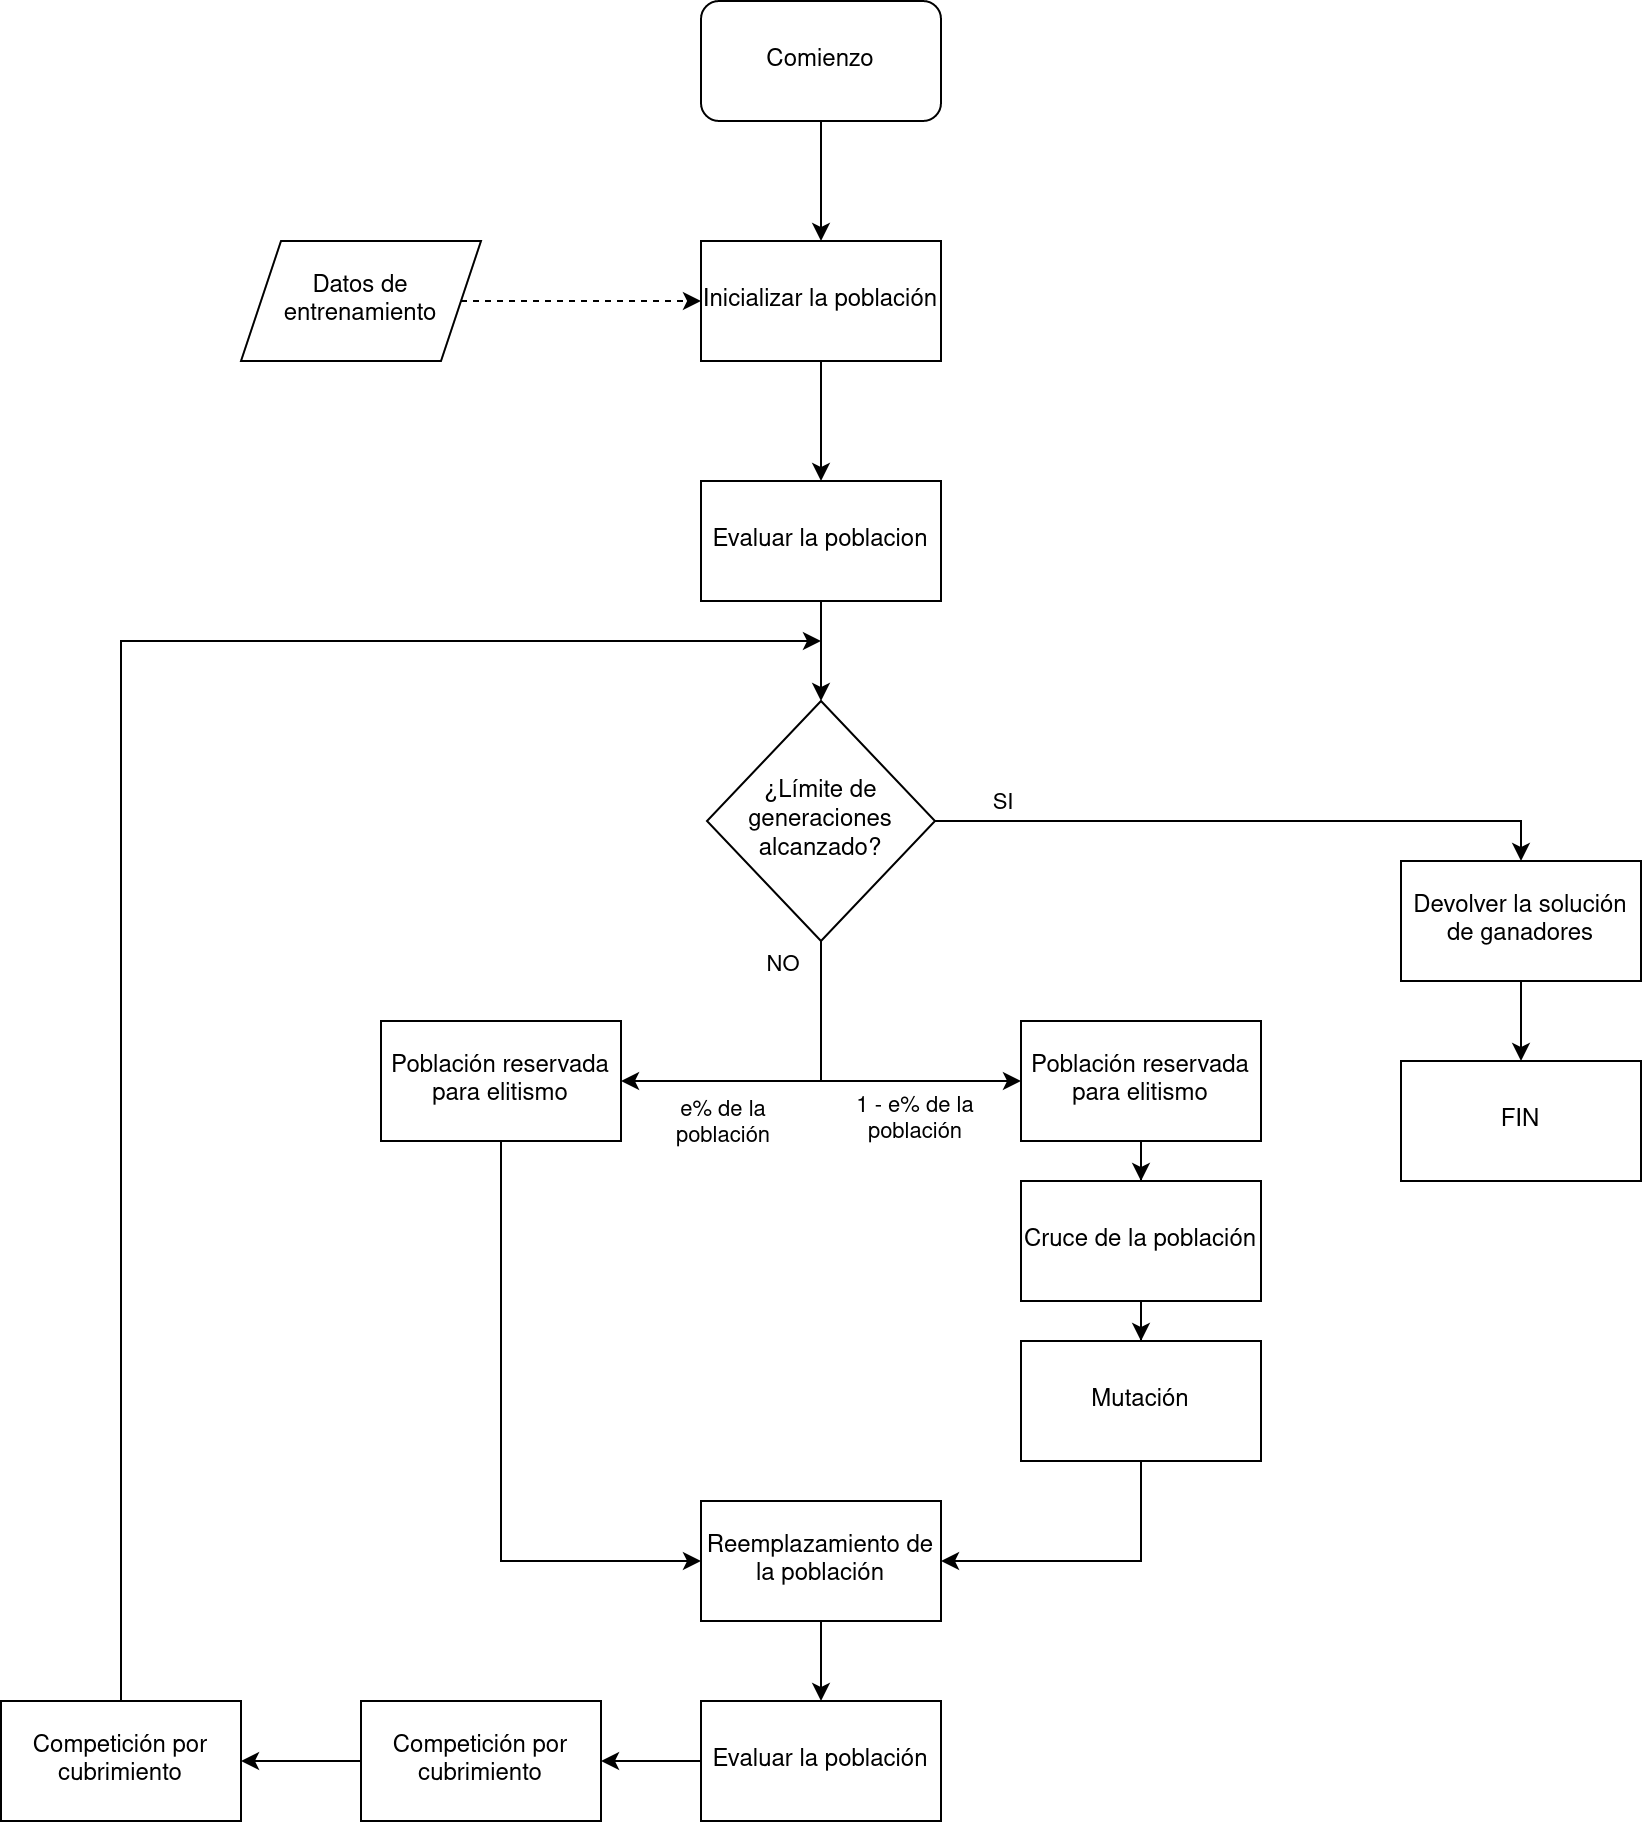
\includegraphics[width = \textwidth]{algoritmo_tan.png}
    \caption{Esquema del algoritmo de Tan.}
	 \label{fig:algoritmo_tan}
\end{figure}

Al igual que en el caso anterior, sigue el esquema de Michigan, ejecutando $n$ veces el algoritmo para un problema de $n$ clases.

\newpage

\subsubsection{Algoritmo de Bojarczuk}


El algoritmo de Bojarczuk \cite{algoritmoBojarczuk} se propuso en 2004 como una nueva propuesta de Programación Genética utilizando una gramática, además de un nuevo enfoque al representar los individuos de la población.

En esta propuesta se utiliza un híbrido entre el enfoque de Michigan y el enfoque de Pittsburgh. En lugar de tener como individuos de la población reglas por separado, o conjuntos completos de reglas, un individuo de la población puede ser un conjunto de reglas, pero solo si dichas reglas tienen el mismo consecuente, es decir, sirven para predecir la misma clase. De esta forma esto les permite hacer un algoritmo más eficiente, ya que no será necesario ejecutarlo $n$ veces para problemas con $n$ clases. Esto puede parecer que se trata del enfoque de Pittsburgh modificado, sin embargo hay que distinguir que un individuo no representa una solución al problema, únicamente la solución al problema para clasificar una de las $n$ clases, por lo tanto la solución al problema será un conjunto de, al menos, $k$ individuos de la población.

En el artículo de la propuesta también discuten la gramática a utilizar, los operadores de dicha gramática, así como las operaciones de cruce y mutación, que son las mismas que las comentadas en apartados anteriores, donde simplemente se sigue la gramática propuesta que simplemente se trata de restricciones en los operadores a utilizar dependiendo de los tipos de datos de los atributos y nodos.

En resumen son las siguientes restricciones sintácticas:

\begin{enumerate}
	\item Un nodo hoja solo puede tener como padre los operadores ``='' o ``!='' si es un atributo categórico y ``<='' o ``>'' si es un atributo continuo.
	\item Un nodo interno con un operador relacional solo puede tener como padre un nodo con un operador lógico (AND o OR).
	\item Un nodo con un operador lógico solo puede tener como padre un nodo con un operador lógico.
	\item Un nodo con el operador lógico OR solo puede tener como padre otro nodo con el operador lógico OR.
	\item Un atributo solo puede aparecer una única vez en el antecedente de una regla.
\end{enumerate}

Como vemos, con estas restricciones establecidas en la gramática por defecto que ofrecen (solo con dos operaciones lógicas y cuatro operadores de relación), tenemos una gran variedad de posibles reglas a generar.

Con respecto al esquema del algoritmo, sigue un esquema básico de algoritmo evolutivo ya visto anteriormente, y no detallan un esquema concreto en su propuesta.

\newpage

\subsection{Validación de las pruebas}


Uno de los problemas que nos encontramos en los algoritmos de aprendizaje automático es la validación del algoritmo, es decir, como podemos asegurar que nuestro algoritmo realmente funciona, y no se trata de que ha hecho un sobreajuste con los datos con los que ha entrenado y fuera de dichos datos no es capaz de realizar buenas predicciones.

Para comprobar y asegurarnos que los algoritmos son capaces de realizar buenas predicciones fuera de los datos con los que ha entrenado utilizaremos validación cruzada con $k$ iteraciones.

Este método consiste en dividir el conjunto de entrenamiento en $k$ partes de mismo tamaño, de forma que realizaremos $k$ iteraciones para entrenar nuestro modelo. En cada iteración utilizaremos una de estas partes como conjunto de validación y las otras $k - 1$ partes como conjunto de entrenamiento, de forma que el algoritmo no haya entrenado con esa parte de validación. Finalmente para obtener el error del algoritmo para dicho conjunto de datos utilizaremos la media del error en los distintos conjuntos de validación de cada iteración.

Es importante destacar que antes de hacer las separaciones en $k$ subconjuntos de datos el conjunto de entrenamiento se reordenará de forma aleatoria para evitar que un conjunto en el que los datos estén ordenados por clase se excluya del entrenamiento cierta clase, porque todas sus muestras están en el conjunto de validación.

De esta forma podremos obtener un valor del error del algoritmo para unos datos con los que no ha entrenado, a la vez que comprobamos que nuestro algoritmo es capaz de ajustarse bien o no a un conjunto de datos.


\begin{figure}[H]
    \centering

	 \begin{subfigure}[b]{\textwidth}
		\centering
		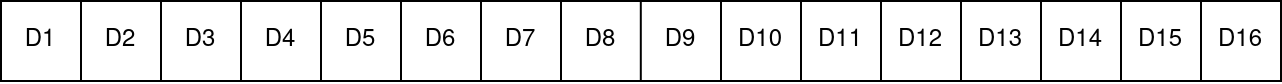
\includegraphics[width=0.8\textwidth]{cross_validation/conjunto_datos.png}
		\caption{Ejemplo de un conjunto de 16 datos.}
	  \label{fig:ej_16_datos}
   \end{subfigure}
	\vspace{1cm}

	 \begin{subfigure}[b]{\textwidth}
		 \centering
		 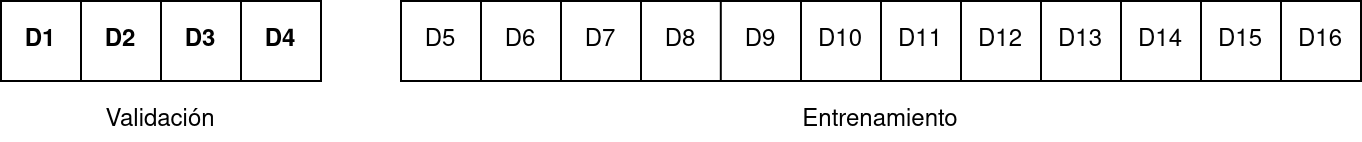
\includegraphics[width=0.8\textwidth]{cross_validation/iteracion1.png}
 		 \caption{Separación entre validación y entrenamiento en la primera iteración.}
 	    \label{fig:cv_iteracion1}
	 \end{subfigure}
	 \vspace{1cm}

	\begin{subfigure}[b]{\textwidth}
		 \centering
		 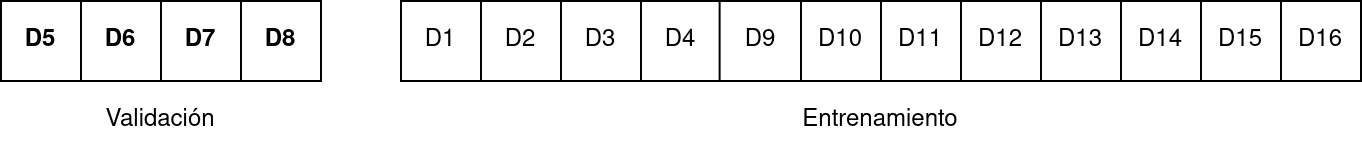
\includegraphics[width=0.8\textwidth]{cross_validation/iteracion2.png}
 		 \caption{Separación entre validación y entrenamiento en la segunda iteración.}
 	    \label{fig:cv_iteracion2}
   \end{subfigure}
	\vspace{1cm}

	\begin{subfigure}[b]{\textwidth}
		 \centering
		 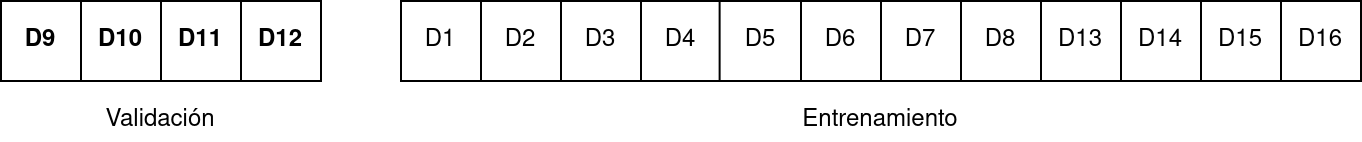
\includegraphics[width=0.8\textwidth]{cross_validation/iteracion3.png}
 		 \caption{Separación entre validación y entrenamiento en la tercera iteración.}
 	    \label{fig:cv_iteracion3}
	\end{subfigure}
	\vspace{1cm}

	\begin{subfigure}[b]{\textwidth}
		 \centering
		 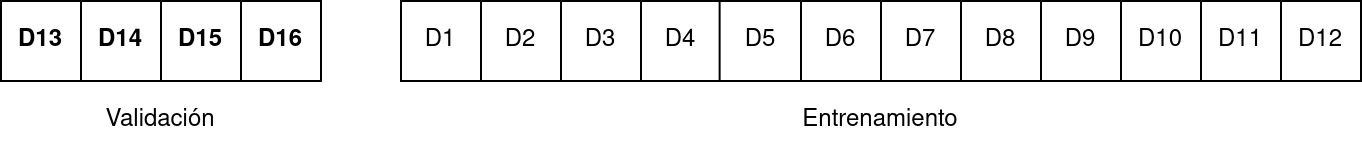
\includegraphics[width=0.8\textwidth]{cross_validation/iteracion4.png}
 		 \caption{Separación entre validación y entrenamiento en la cuarta iteración.}
 	    \label{fig:cv_iteracion4}
	\end{subfigure}

	\caption{Ejemplo de validación cruzada de 4 iteraciones.}
	\label{fig:4-cv-ejemplo}
\end{figure}


En nuestro caso utilizaremos una validación cruzada de cinco folds para validación, además de contar con un conjunto de test en el que no se ha aplicado el sobremuestro, para comprobar como se comporta con datos reales y sin replicar.


\newpage

\subsection{Funciones de evaluación}

De cara a evaluar los algoritmos necesitaremos una función de evaluación que nos permita saber el error que estamos cometiendo en las estimaciones.

En nuestro caso, al estar ante un problema de clasificación utilizaremos las siguientes:

\begin{itemize}
	\item Precisión.
	% \item Área bajo la curva ROC.
	\item Error absoluto medio ordinal.
\end{itemize}

\subsubsection{Precisión}

La precisión se trata de una medida de evaluación bastante simple, es el número de observaciones clasificadas correctamente entre el número de observaciones total. Este ratio nos ofrece información sobre cuantas observaciones estamos clasificando de forma correcta:

\begin{figure}[H]
	 \centering
	 $$ Accuracy = \frac{\text{N. de observaciones clasificadas de forma correcta}}{\text{N. total de observaciones}} $$
	 \caption{Fórmula para calcular la precisión.}
	\label{fig:Accuracy}
\end{figure}

\subsubsection{Error absoluto medio ordinal}

El error absoluto medio ordinal (OMAE por sus siglas en inglés) se trata de medir la diferencia entre dos valores, en nuestro caso los valores obtenidos y los valores esperados. En principio este error se utiliza en regresión, sin embargo, debido a que nuestro problema es un problema de clasificación ordinal (el orden de las clases tiene un significado e importancia a la hora de equivocarnos), podemos aplicar esta métrica a nuestro problema asignando a cada clase un orden, en nuestro caso del 1 al 10.

\begin{figure}[H]
	 \centering
	 $$ OMAE = \frac{\sum_{i = 1}^{n}|\hat{Y_i} - Y_i|}{n} $$
	 \caption{Fórmula para calcular el error absoluto medio ordinal, donde $\hat{Y_i}$ son las etiquetas predichas y $Y_i$ son las etiquetas reales.}
	\label{fig:MAE}
\end{figure}


\newpage
